\documentclass{article}\usepackage{graphicx, color}
%% maxwidth is the original width if it is less than linewidth
%% otherwise use linewidth (to make sure the graphics do not exceed the margin)
\makeatletter
\def\maxwidth{ %
  \ifdim\Gin@nat@width>\linewidth
    \linewidth
  \else
    \Gin@nat@width
  \fi
}
\makeatother

\IfFileExists{upquote.sty}{\usepackage{upquote}}{}
\definecolor{fgcolor}{rgb}{0.2, 0.2, 0.2}
\newcommand{\hlnumber}[1]{\textcolor[rgb]{0,0,0}{#1}}%
\newcommand{\hlfunctioncall}[1]{\textcolor[rgb]{0.501960784313725,0,0.329411764705882}{\textbf{#1}}}%
\newcommand{\hlstring}[1]{\textcolor[rgb]{0.6,0.6,1}{#1}}%
\newcommand{\hlkeyword}[1]{\textcolor[rgb]{0,0,0}{\textbf{#1}}}%
\newcommand{\hlargument}[1]{\textcolor[rgb]{0.690196078431373,0.250980392156863,0.0196078431372549}{#1}}%
\newcommand{\hlcomment}[1]{\textcolor[rgb]{0.180392156862745,0.6,0.341176470588235}{#1}}%
\newcommand{\hlroxygencomment}[1]{\textcolor[rgb]{0.43921568627451,0.47843137254902,0.701960784313725}{#1}}%
\newcommand{\hlformalargs}[1]{\textcolor[rgb]{0.690196078431373,0.250980392156863,0.0196078431372549}{#1}}%
\newcommand{\hleqformalargs}[1]{\textcolor[rgb]{0.690196078431373,0.250980392156863,0.0196078431372549}{#1}}%
\newcommand{\hlassignement}[1]{\textcolor[rgb]{0,0,0}{\textbf{#1}}}%
\newcommand{\hlpackage}[1]{\textcolor[rgb]{0.588235294117647,0.709803921568627,0.145098039215686}{#1}}%
\newcommand{\hlslot}[1]{\textit{#1}}%
\newcommand{\hlsymbol}[1]{\textcolor[rgb]{0,0,0}{#1}}%
\newcommand{\hlprompt}[1]{\textcolor[rgb]{0.2,0.2,0.2}{#1}}%

\usepackage{framed}
\makeatletter
\newenvironment{kframe}{%
 \def\at@end@of@kframe{}%
 \ifinner\ifhmode%
  \def\at@end@of@kframe{\end{minipage}}%
  \begin{minipage}{\columnwidth}%
 \fi\fi%
 \def\FrameCommand##1{\hskip\@totalleftmargin \hskip-\fboxsep
 \colorbox{shadecolor}{##1}\hskip-\fboxsep
     % There is no \\@totalrightmargin, so:
     \hskip-\linewidth \hskip-\@totalleftmargin \hskip\columnwidth}%
 \MakeFramed {\advance\hsize-\width
   \@totalleftmargin\z@ \linewidth\hsize
   \@setminipage}}%
 {\par\unskip\endMakeFramed%
 \at@end@of@kframe}
\makeatother

\definecolor{shadecolor}{rgb}{.97, .97, .97}
\definecolor{messagecolor}{rgb}{0, 0, 0}
\definecolor{warningcolor}{rgb}{1, 0, 1}
\definecolor{errorcolor}{rgb}{1, 0, 0}
\newenvironment{knitrout}{}{} % an empty environment to be redefined in TeX

\usepackage{alltt}



\title{Drawing Graphs for Incidence and Prevalence}
\author{Danny Kaplan}
\date{Sept. 8, 2010}
\begin{document}

\maketitle

Drawing graphs showing the progression of individuals through sickness
and death (or loss to follow-up), to help students estimate prevalence
and incidence.

Basic idea, for each person, generate a probability of sickness,
death, or loss.  Draw a line graph appropriately

Functions for getting sick, dying, or getting lost to follow up:
\begin{knitrout}
\definecolor{shadecolor}{rgb}{0.969, 0.969, 0.969}\color{fgcolor}\begin{kframe}
\begin{alltt}
sick = \hlfunctioncall{function}(rate = 0.07) \{
    \hlfunctioncall{rexp}(1, rate = rate)
\}
loss = \hlfunctioncall{function}(rate = 0.02, lockout = 0.5) \{
    lockout + \hlfunctioncall{rexp}(1, rate = rate)
\}
death = \hlfunctioncall{function}(rate = 0.05) \{
    \hlfunctioncall{rexp}(1, rate = rate)
\}
\end{alltt}
\end{kframe}
\end{knitrout}


Put these together for one person, graphing out the result:
\begin{knitrout}
\definecolor{shadecolor}{rgb}{0.969, 0.969, 0.969}\color{fgcolor}\begin{kframe}
\begin{alltt}
one.person = \hlfunctioncall{function}(loc=1) \{
  S=\hlfunctioncall{sick}(); L=\hlfunctioncall{loss}(); D=\hlfunctioncall{death}()
  \hlfunctioncall{if}( S <= L & S <= D ) \{
    \hlcomment{# they got sick first.}
    \hlfunctioncall{lines}( \hlfunctioncall{c}(0,\hlfunctioncall{min}(10,S)), \hlfunctioncall{c}(loc,loc), col=\hlstring{"gray"}, lwd=3 );
    \hlcomment{# now figure out when they die or get lost.}
    L = \hlfunctioncall{loss}(); D=\hlfunctioncall{death}(rate=.3); \hlcomment{# a higher death rate}
    \hlfunctioncall{if} (S < 10 )
      \hlfunctioncall{lines}( \hlfunctioncall{c}(S,\hlfunctioncall{min}(10,S+\hlfunctioncall{min}(D,L))), \hlfunctioncall{c}(loc,loc), col=\hlstring{"red"}, lwd=5 );
  \}
  else \{
    S = 0; \hlcomment{# they never got sick}
    \hlfunctioncall{lines}( \hlfunctioncall{c}(0,\hlfunctioncall{min}(10,\hlfunctioncall{min}(D,L))), \hlfunctioncall{c}(loc,loc), col=\hlstring{"gray"}, lwd=3 );
  \}
  \hlfunctioncall{if}( L < D ) \{
    \hlfunctioncall{text}( S+L+.2, loc, \hlstring{"?"}, col=\hlstring{'red'});
  \}
  else \{
    \hlfunctioncall{text}( S+D, loc, \hlstring{"X"}, col=\hlstring{"black"});
  \}
\}
\end{alltt}
\end{kframe}
\end{knitrout}



Plot out a lot of them.
\begin{knitrout}
\definecolor{shadecolor}{rgb}{0.969, 0.969, 0.969}\color{fgcolor}\begin{kframe}
\begin{alltt}
show.population = \hlfunctioncall{function}(n) \{
    \hlfunctioncall{plot}(1:10, xlim = \hlfunctioncall{c}(0, 10), ylim = \hlfunctioncall{c}(0, n), type = \hlstring{"n"}, yaxt = \hlstring{"n"}, ylab = \hlstring{"People"}, 
        xlab = \hlstring{"Years of Follow Up"})
    \hlfunctioncall{for} (k in 1:n) \hlfunctioncall{one.person}(k)
\}
\end{alltt}
\end{kframe}
\end{knitrout}


\section{For the Groups to Work On}

\begin{knitrout}
\definecolor{shadecolor}{rgb}{0.969, 0.969, 0.969}\color{fgcolor}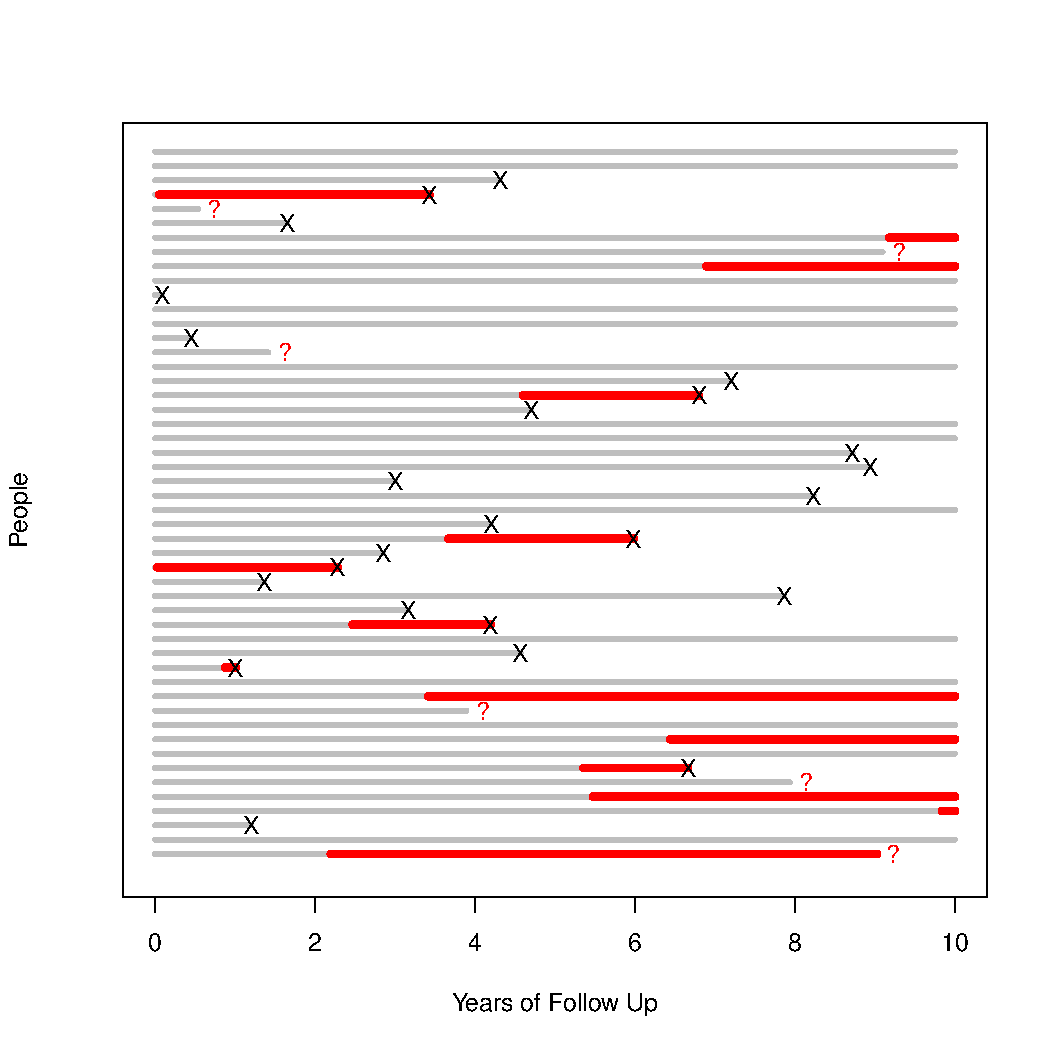
\includegraphics[width=6in]{figure/one} 
\end{knitrout}


\begin{knitrout}
\definecolor{shadecolor}{rgb}{0.969, 0.969, 0.969}\color{fgcolor}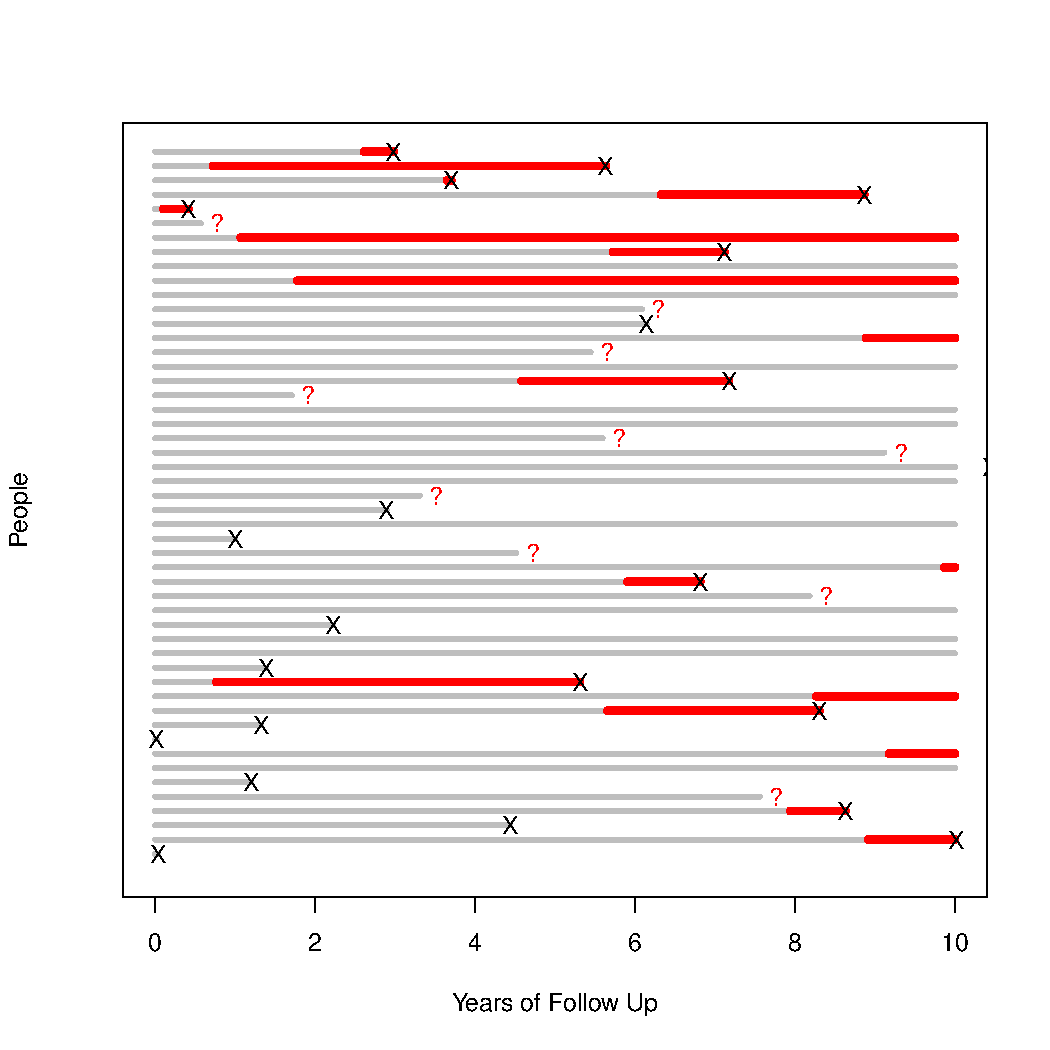
\includegraphics[width=6in]{figure/two} 
\end{knitrout}


\begin{knitrout}
\definecolor{shadecolor}{rgb}{0.969, 0.969, 0.969}\color{fgcolor}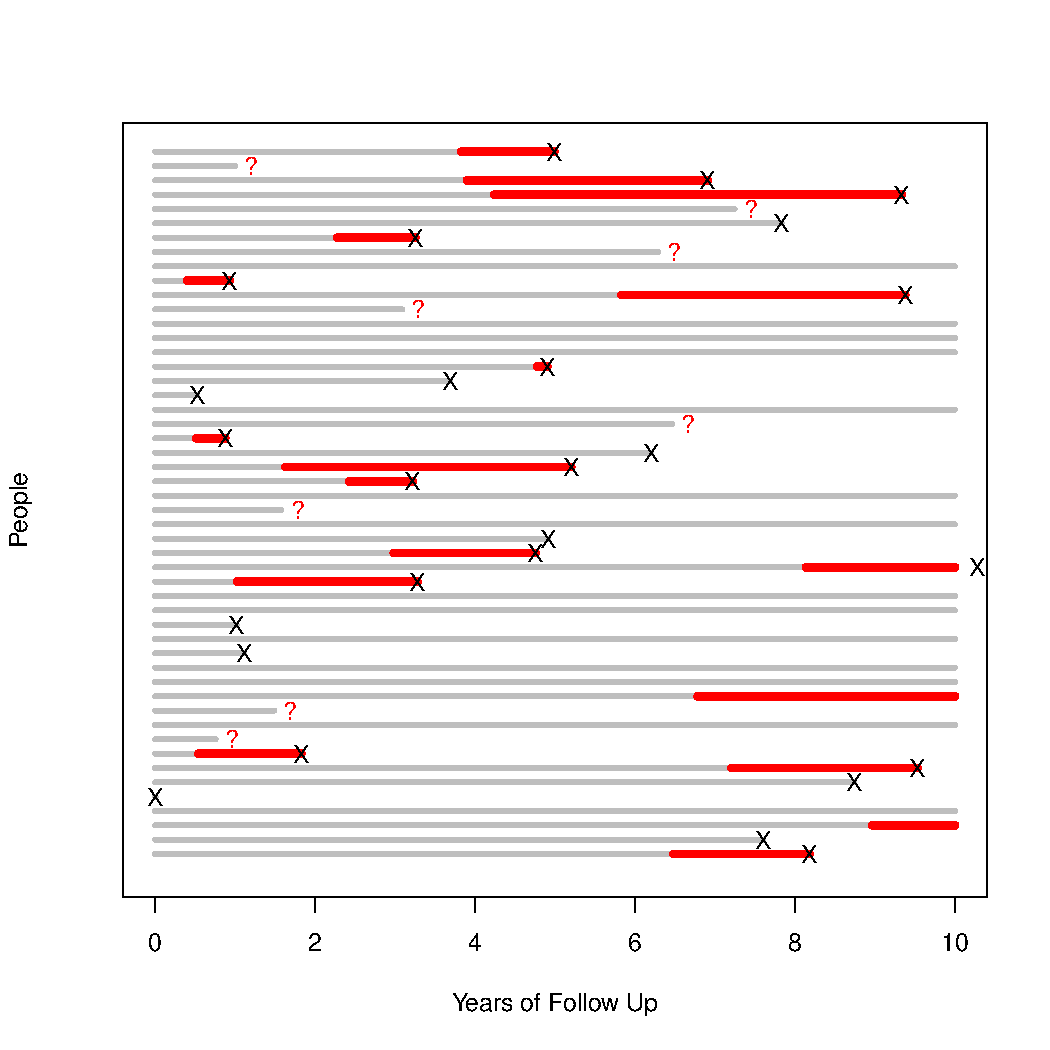
\includegraphics[width=6in]{figure/three} 
\end{knitrout}


\begin{knitrout}
\definecolor{shadecolor}{rgb}{0.969, 0.969, 0.969}\color{fgcolor}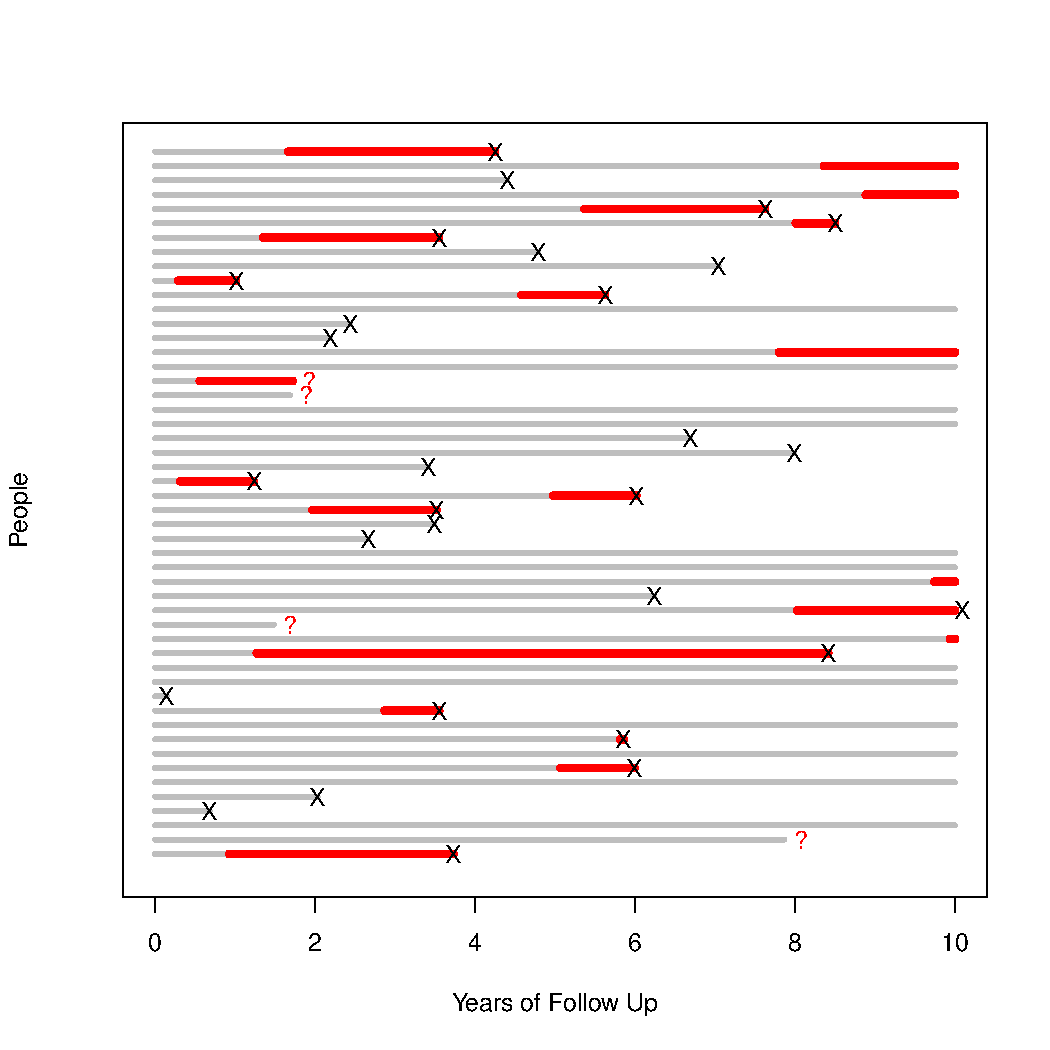
\includegraphics[width=6in]{figure/four} 
\end{knitrout}


\begin{knitrout}
\definecolor{shadecolor}{rgb}{0.969, 0.969, 0.969}\color{fgcolor}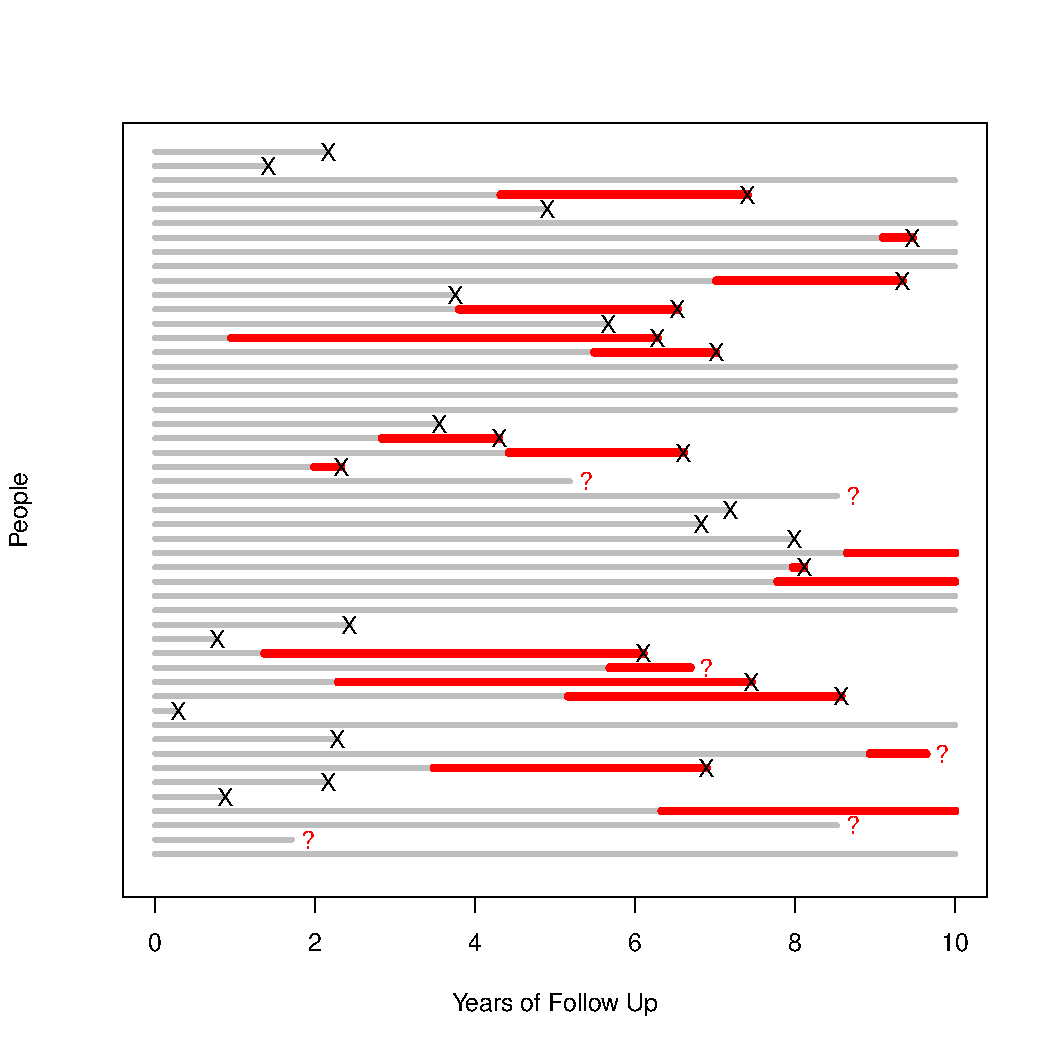
\includegraphics[width=6in]{figure/five} 
\end{knitrout}


\begin{knitrout}
\definecolor{shadecolor}{rgb}{0.969, 0.969, 0.969}\color{fgcolor}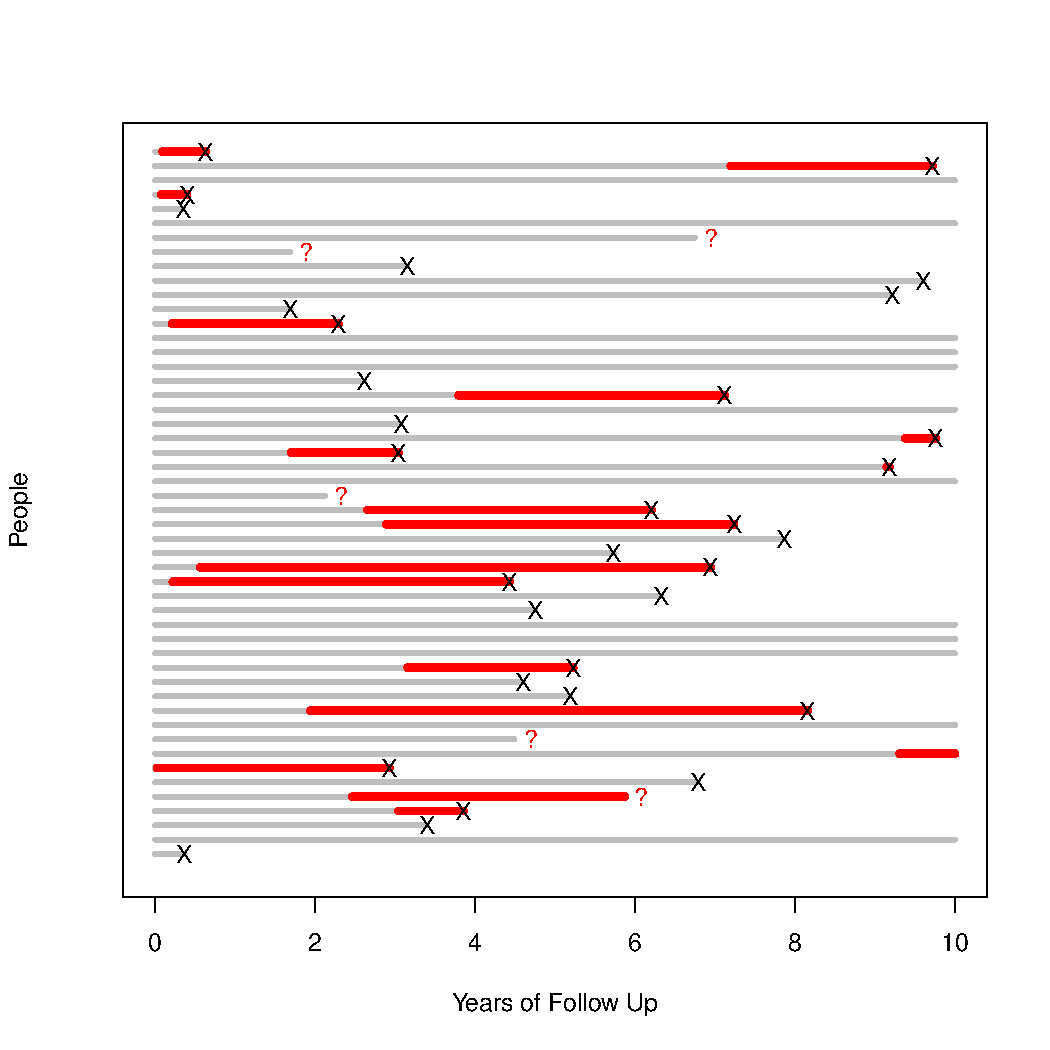
\includegraphics[width=6in]{figure/six} 
\end{knitrout}


\begin{knitrout}
\definecolor{shadecolor}{rgb}{0.969, 0.969, 0.969}\color{fgcolor}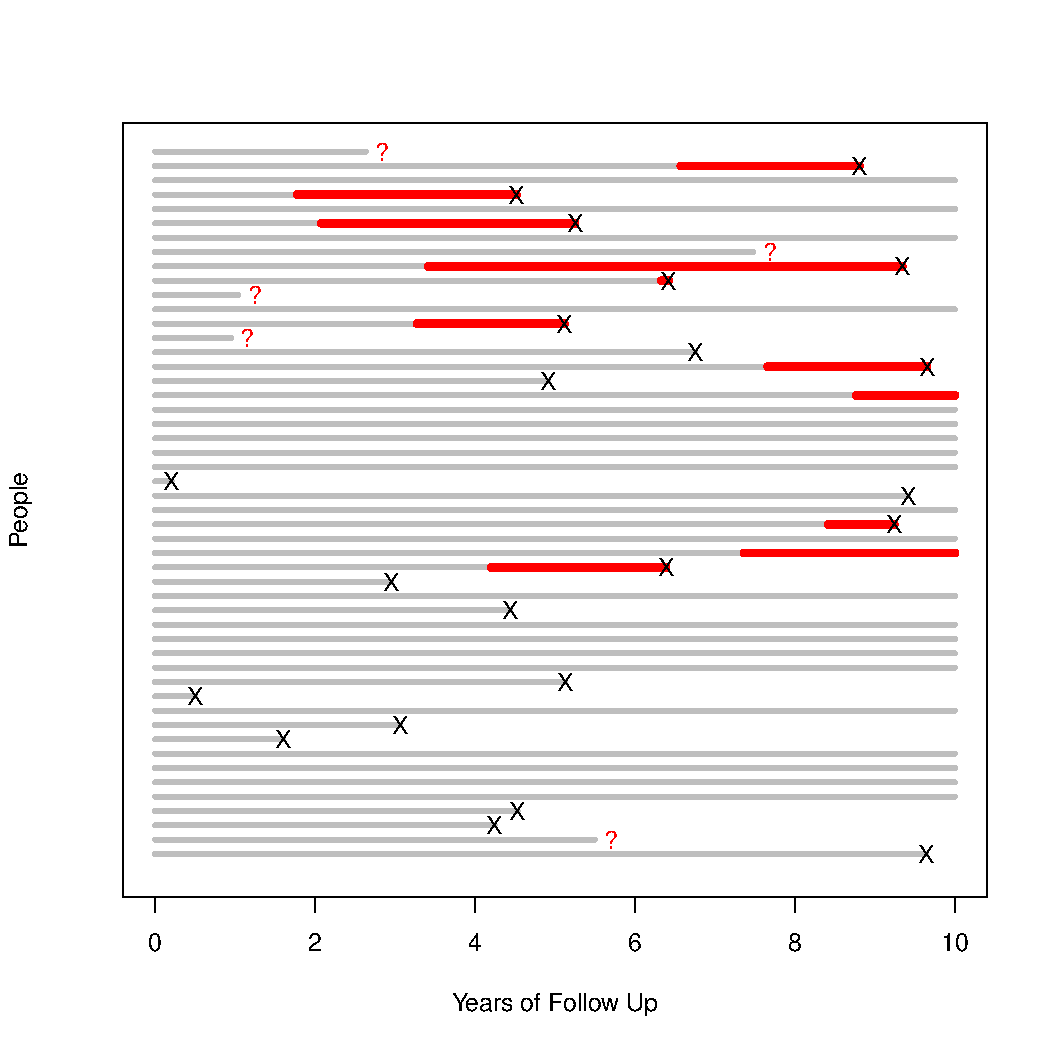
\includegraphics[width=6in]{figure/seven} 
\end{knitrout}


\begin{knitrout}
\definecolor{shadecolor}{rgb}{0.969, 0.969, 0.969}\color{fgcolor}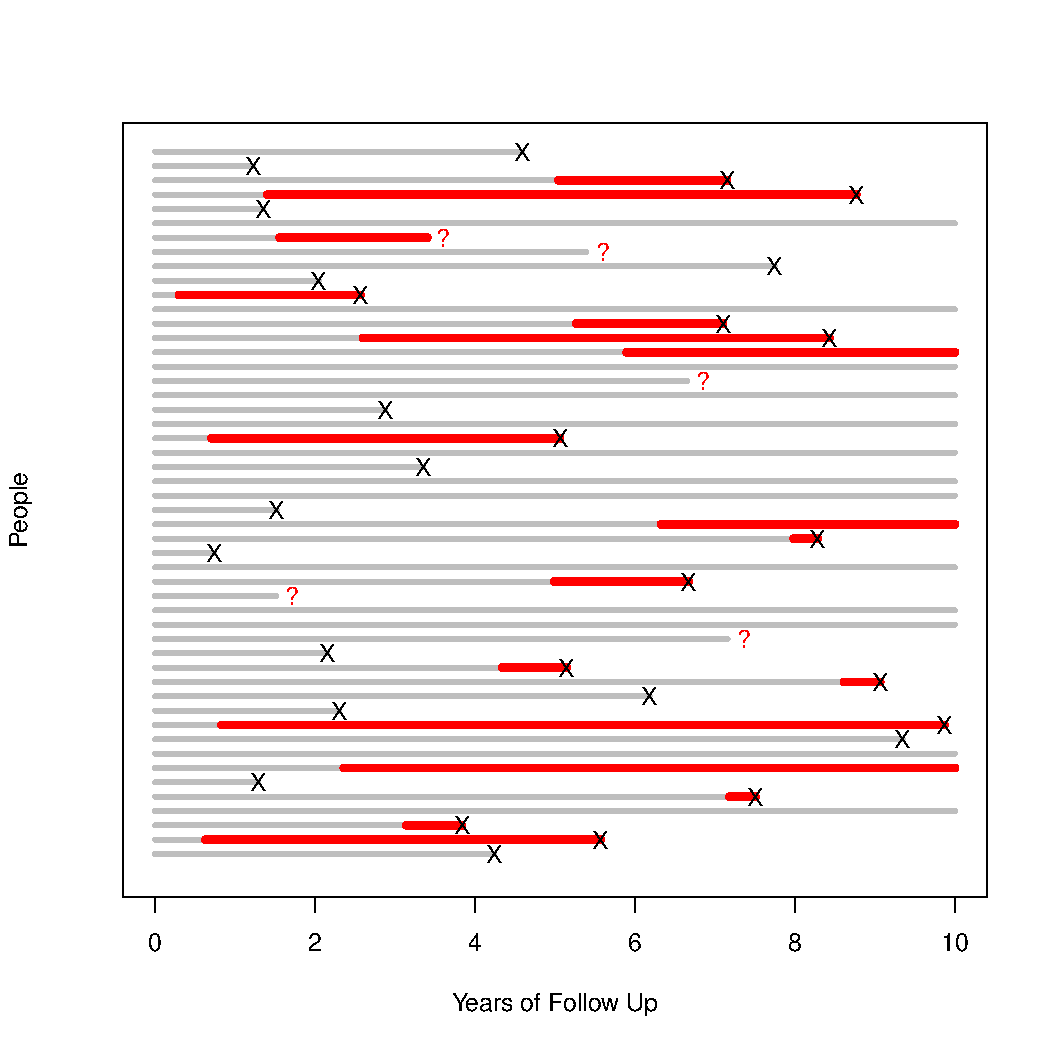
\includegraphics[width=6in]{figure/eight} 
\end{knitrout}


\begin{knitrout}
\definecolor{shadecolor}{rgb}{0.969, 0.969, 0.969}\color{fgcolor}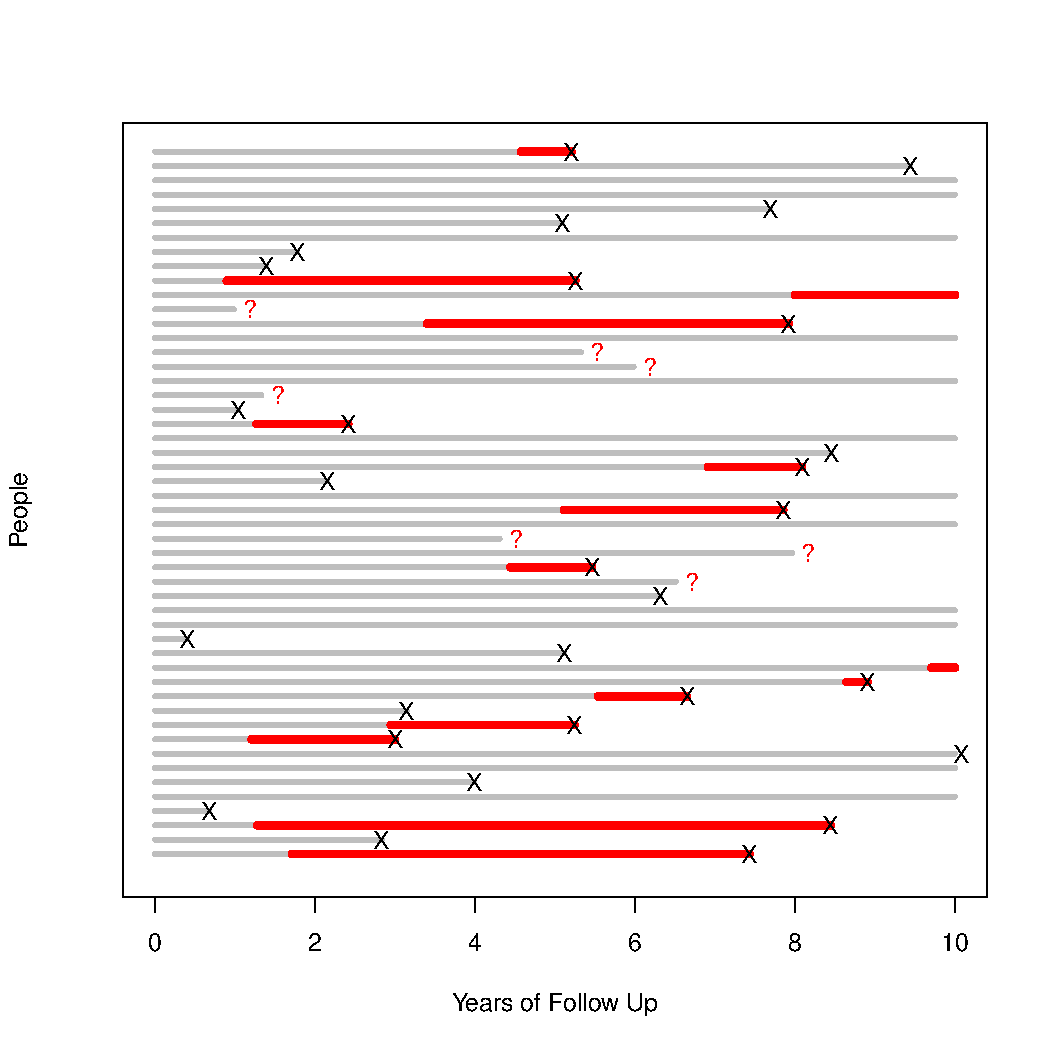
\includegraphics[width=6in]{figure/nine} 
\end{knitrout}


\begin{knitrout}
\definecolor{shadecolor}{rgb}{0.969, 0.969, 0.969}\color{fgcolor}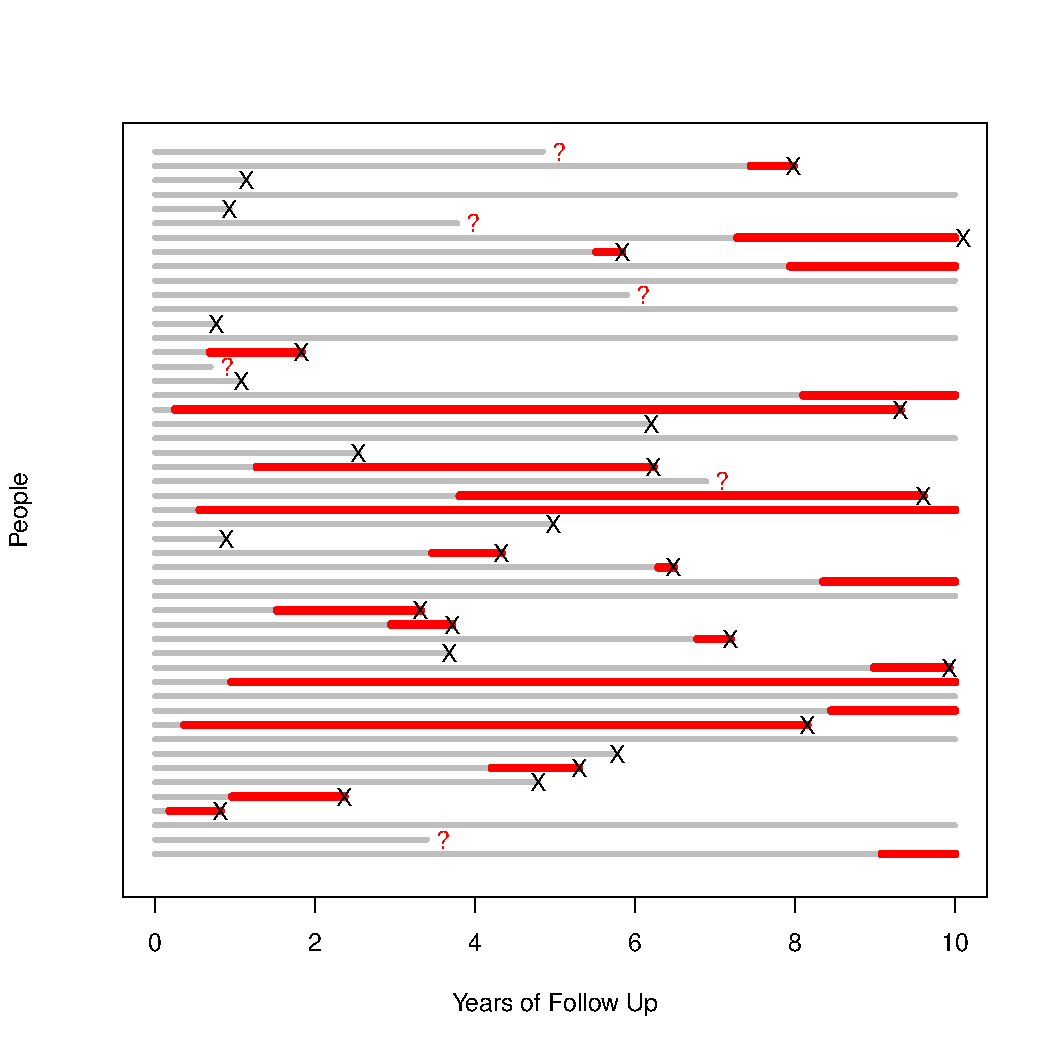
\includegraphics[width=6in]{figure/ten} 
\end{knitrout}


\section{For the In-Class Explanation}
\begin{knitrout}
\definecolor{shadecolor}{rgb}{0.969, 0.969, 0.969}\color{fgcolor}\begin{kframe}
\begin{alltt}
sick = \hlfunctioncall{function}(rate = 0.03) \{
    \hlfunctioncall{rexp}(1, rate = rate)
\}
loss = \hlfunctioncall{function}(rate = 0.01, lockout = 0.5) \{
    lockout + \hlfunctioncall{rexp}(1, rate = rate)
\}
death = \hlfunctioncall{function}(rate = 0.025) \{
    \hlfunctioncall{rexp}(1, rate = rate)
\}
\end{alltt}
\end{kframe}
\end{knitrout}



\begin{knitrout}
\definecolor{shadecolor}{rgb}{0.969, 0.969, 0.969}\color{fgcolor}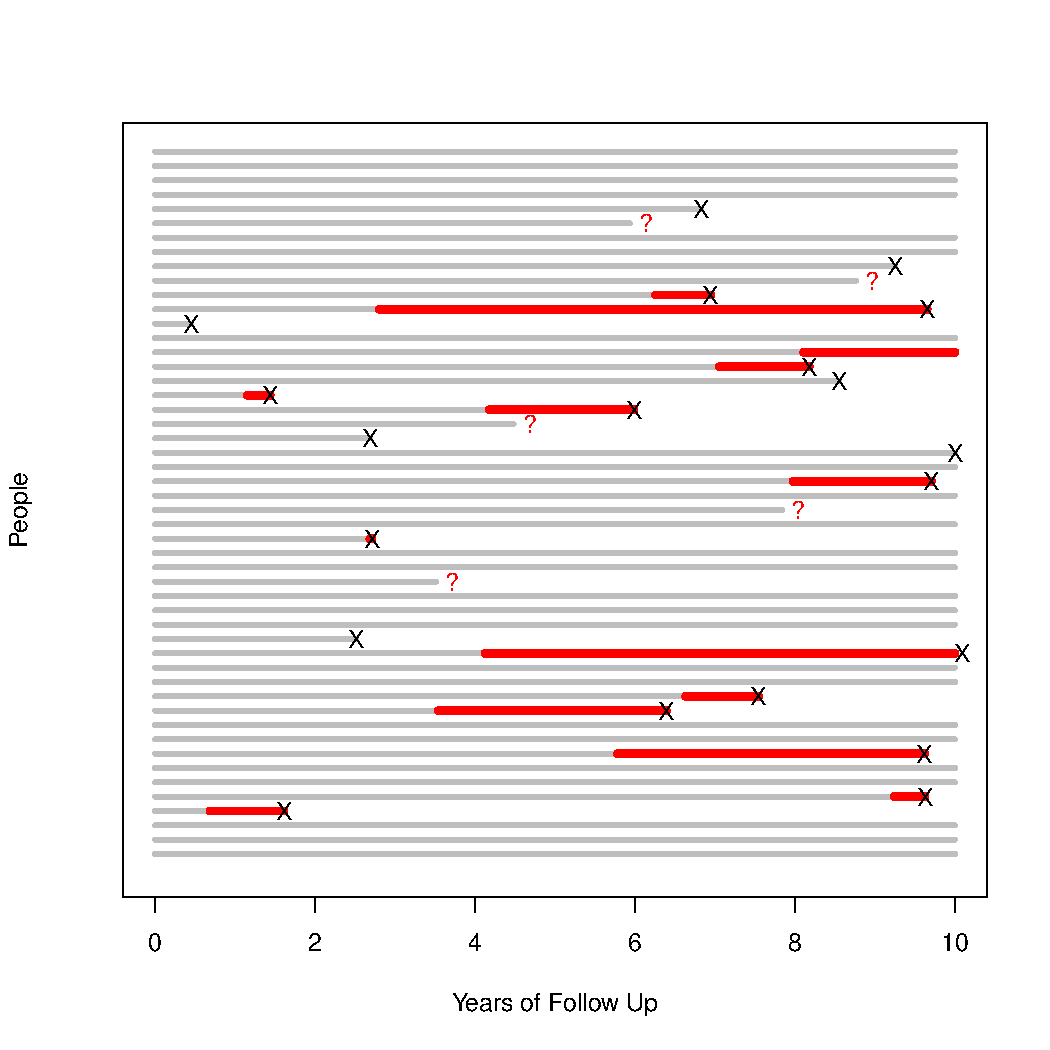
\includegraphics[width=6in]{figure/inclass} 
\end{knitrout}





\end{document}
